%%
%  ******************************************************************************
%  * #file    Szablon_raportu_EN_Latex.tex
%  * #author  Adrian Wójcik   adrian.wojcik(at)put.poznan.pl
%  *          
%  * #commit  Patryk Kościk   koscikpatryk(at)gmail.com
%  *          Modified the template for Projekt przejsciowy purposes          
%  *          
%  * #version 1.0
%  * #date    09-Mar-2022
%  * #brief   PROJPRZEJ
%  *
%  ******************************************************************************
%%  
\documentclass[11pt, a4paper]{article}

\usepackage{SM_template}

% Wypełnijcie te dyrektywy zgodnie z waszym tematem
% \lab      -> NAZWA CZUJNIKA, np.: 'DHT22'
% \comment  -> Króciutki opis co to, np.: 'Cyfrowy budżetowy czujnik temperatury'
%

\lab{TowerPro SG90}
\comment{Serwomechanizm}
\author{Antoni Borowski}
\addbibresource{bib/Serwo.bib}

% Absolutny zakaz dotykania tego tutaj bo jak dotkiecie to coś jebnie
\university{Politechnika Poznańska}
\faculty{Wydział Automatyki, Robotyki i Elektrotechniki}
\institute{Instytut Robotyki i Inteligencji Maszynowej}
\department{Zakład Sterowania i Elektroniki Przemysłowej}

\nocite{}


%%
%
% Początek dokumentu
%
%%
\begin{document}

%% Strona tytułowa %%
\mainpage{{Serwo/front}}
\newpage

\section*{Opis elementu} \addcontentsline{toc}{section}{Wstęp}
Serwomechanizm TowerPro SG-90 to niskonapięciowy serwomotor przeznaczony do wykorzystania przy mikrokontorlerach. Serwomotor to silnik, który umożliwia kontrolowanie dokładnej pozycji wału silnika, prędkości obrotowej lub przyspieszenia. W tym przypadku mamy możliwość kontroli tylko położenia. Moduł może być zasilany wartością napięcia 3-6V, zakres wypełnienia PWM wynosi 500-2400ms.

\begin{figure}[h!]
\centering
\begin{subfigure}{.5\textwidth}
  \centering
  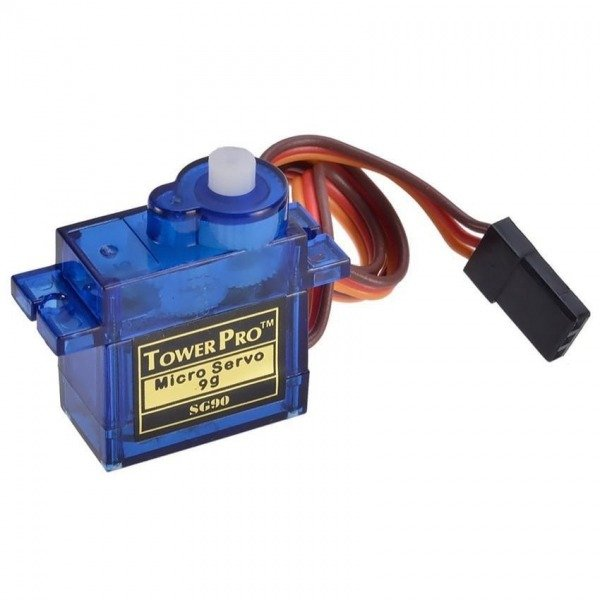
\includegraphics[width=0.9\linewidth]{fig/Serwo/zdj_modułu/fig1.png}
  \caption{Serwomechanizm}
  \label{fig:sub1}
\end{subfigure}%
\begin{subfigure}{.5\textwidth}
  \centering
  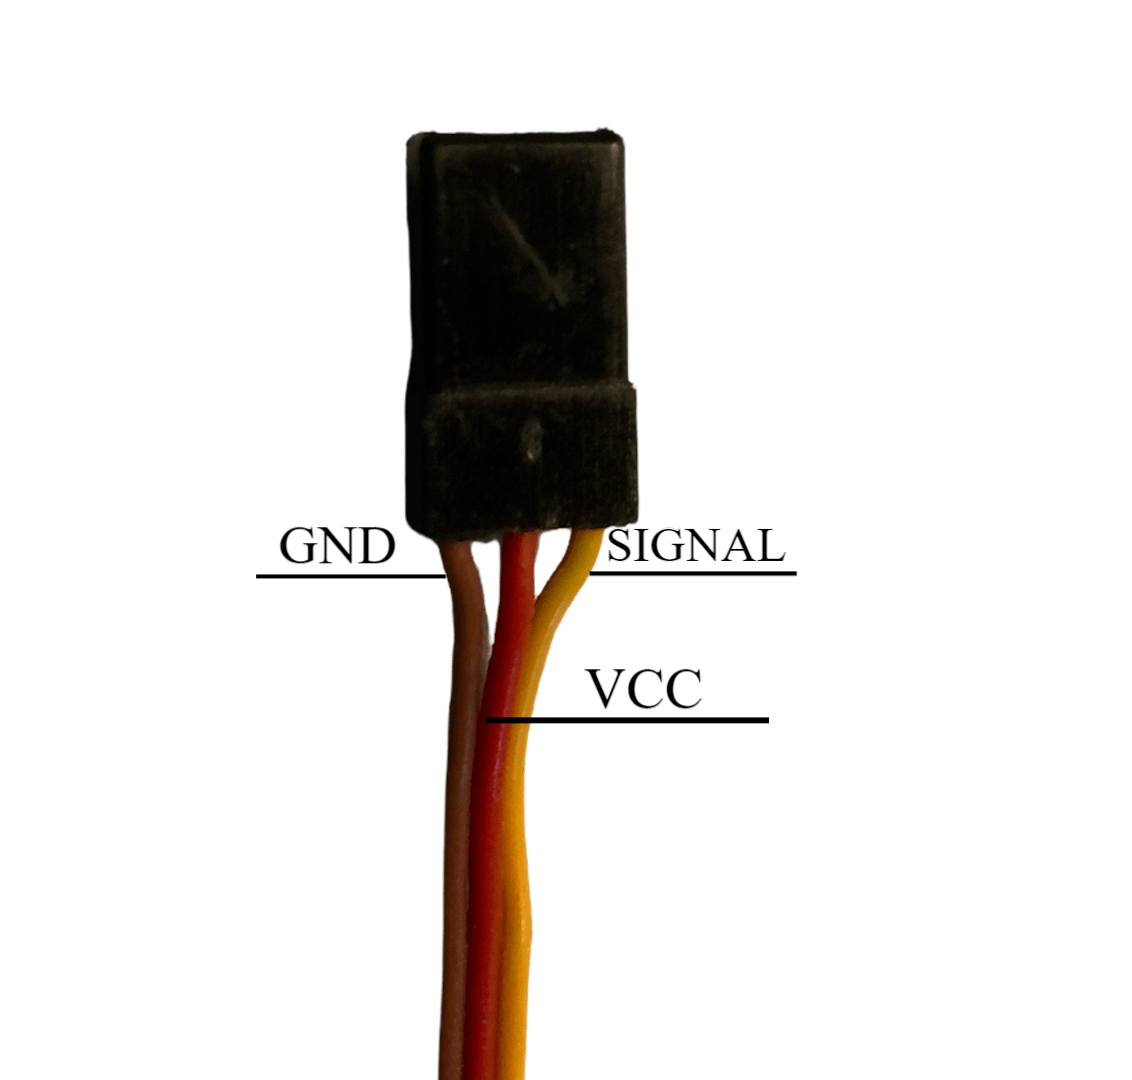
\includegraphics[width=0.9\linewidth]{fig/Serwo/zdj_modułu/kable.png}
  \caption{Wyprowadzenia}
  \label{fig:sub2}
\end{subfigure}
\caption{Poglądowe zdjęcia modułu}
\label{fig:test}
\end{figure}

\newline
Serwomechanizm TowerPro SG-90 ma zakres położenia 180$^{\circ}$, który jest zadawany poprzez zmianę wypełnienia sygnału PWM o częstotliwości 50Hz. Wypełnienie 2\% odpowiada położeniu 0$^{\circ}$, a 12\% położeniu 180$^{\circ}$ - wszystkie wartości pomiędzy są rozmieszczone równomiernie. Moduł ma trzy wyprowadzenia - VCC, GND oraz pin sygnałowy, który będzie podpięty do pinu zegara w płytce Nucleo, by zadawać wartość PWM.
\begin{figure}[h!]
\centering
  \centering
  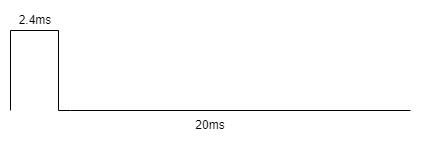
\includegraphics[width=1\linewidth]{fig/Serwo/zasada_dzialania/jeden cykl.png}
  \caption{Przebieg jednego okresu sygnału sterującego przy zadawaniu położenia 180$^{\circ}$}
  \label{fig:sub1}
\end{figure}

\newpage
\section*{Użycie czujnika}
Poniżej przedstawiono podstawowe podłączenie serwomechanizmu do mikroprocesora według oznaczeń z Rys.1(b).
\vspace{0.5cm}
\begin{figure}[h!]
    \centering
    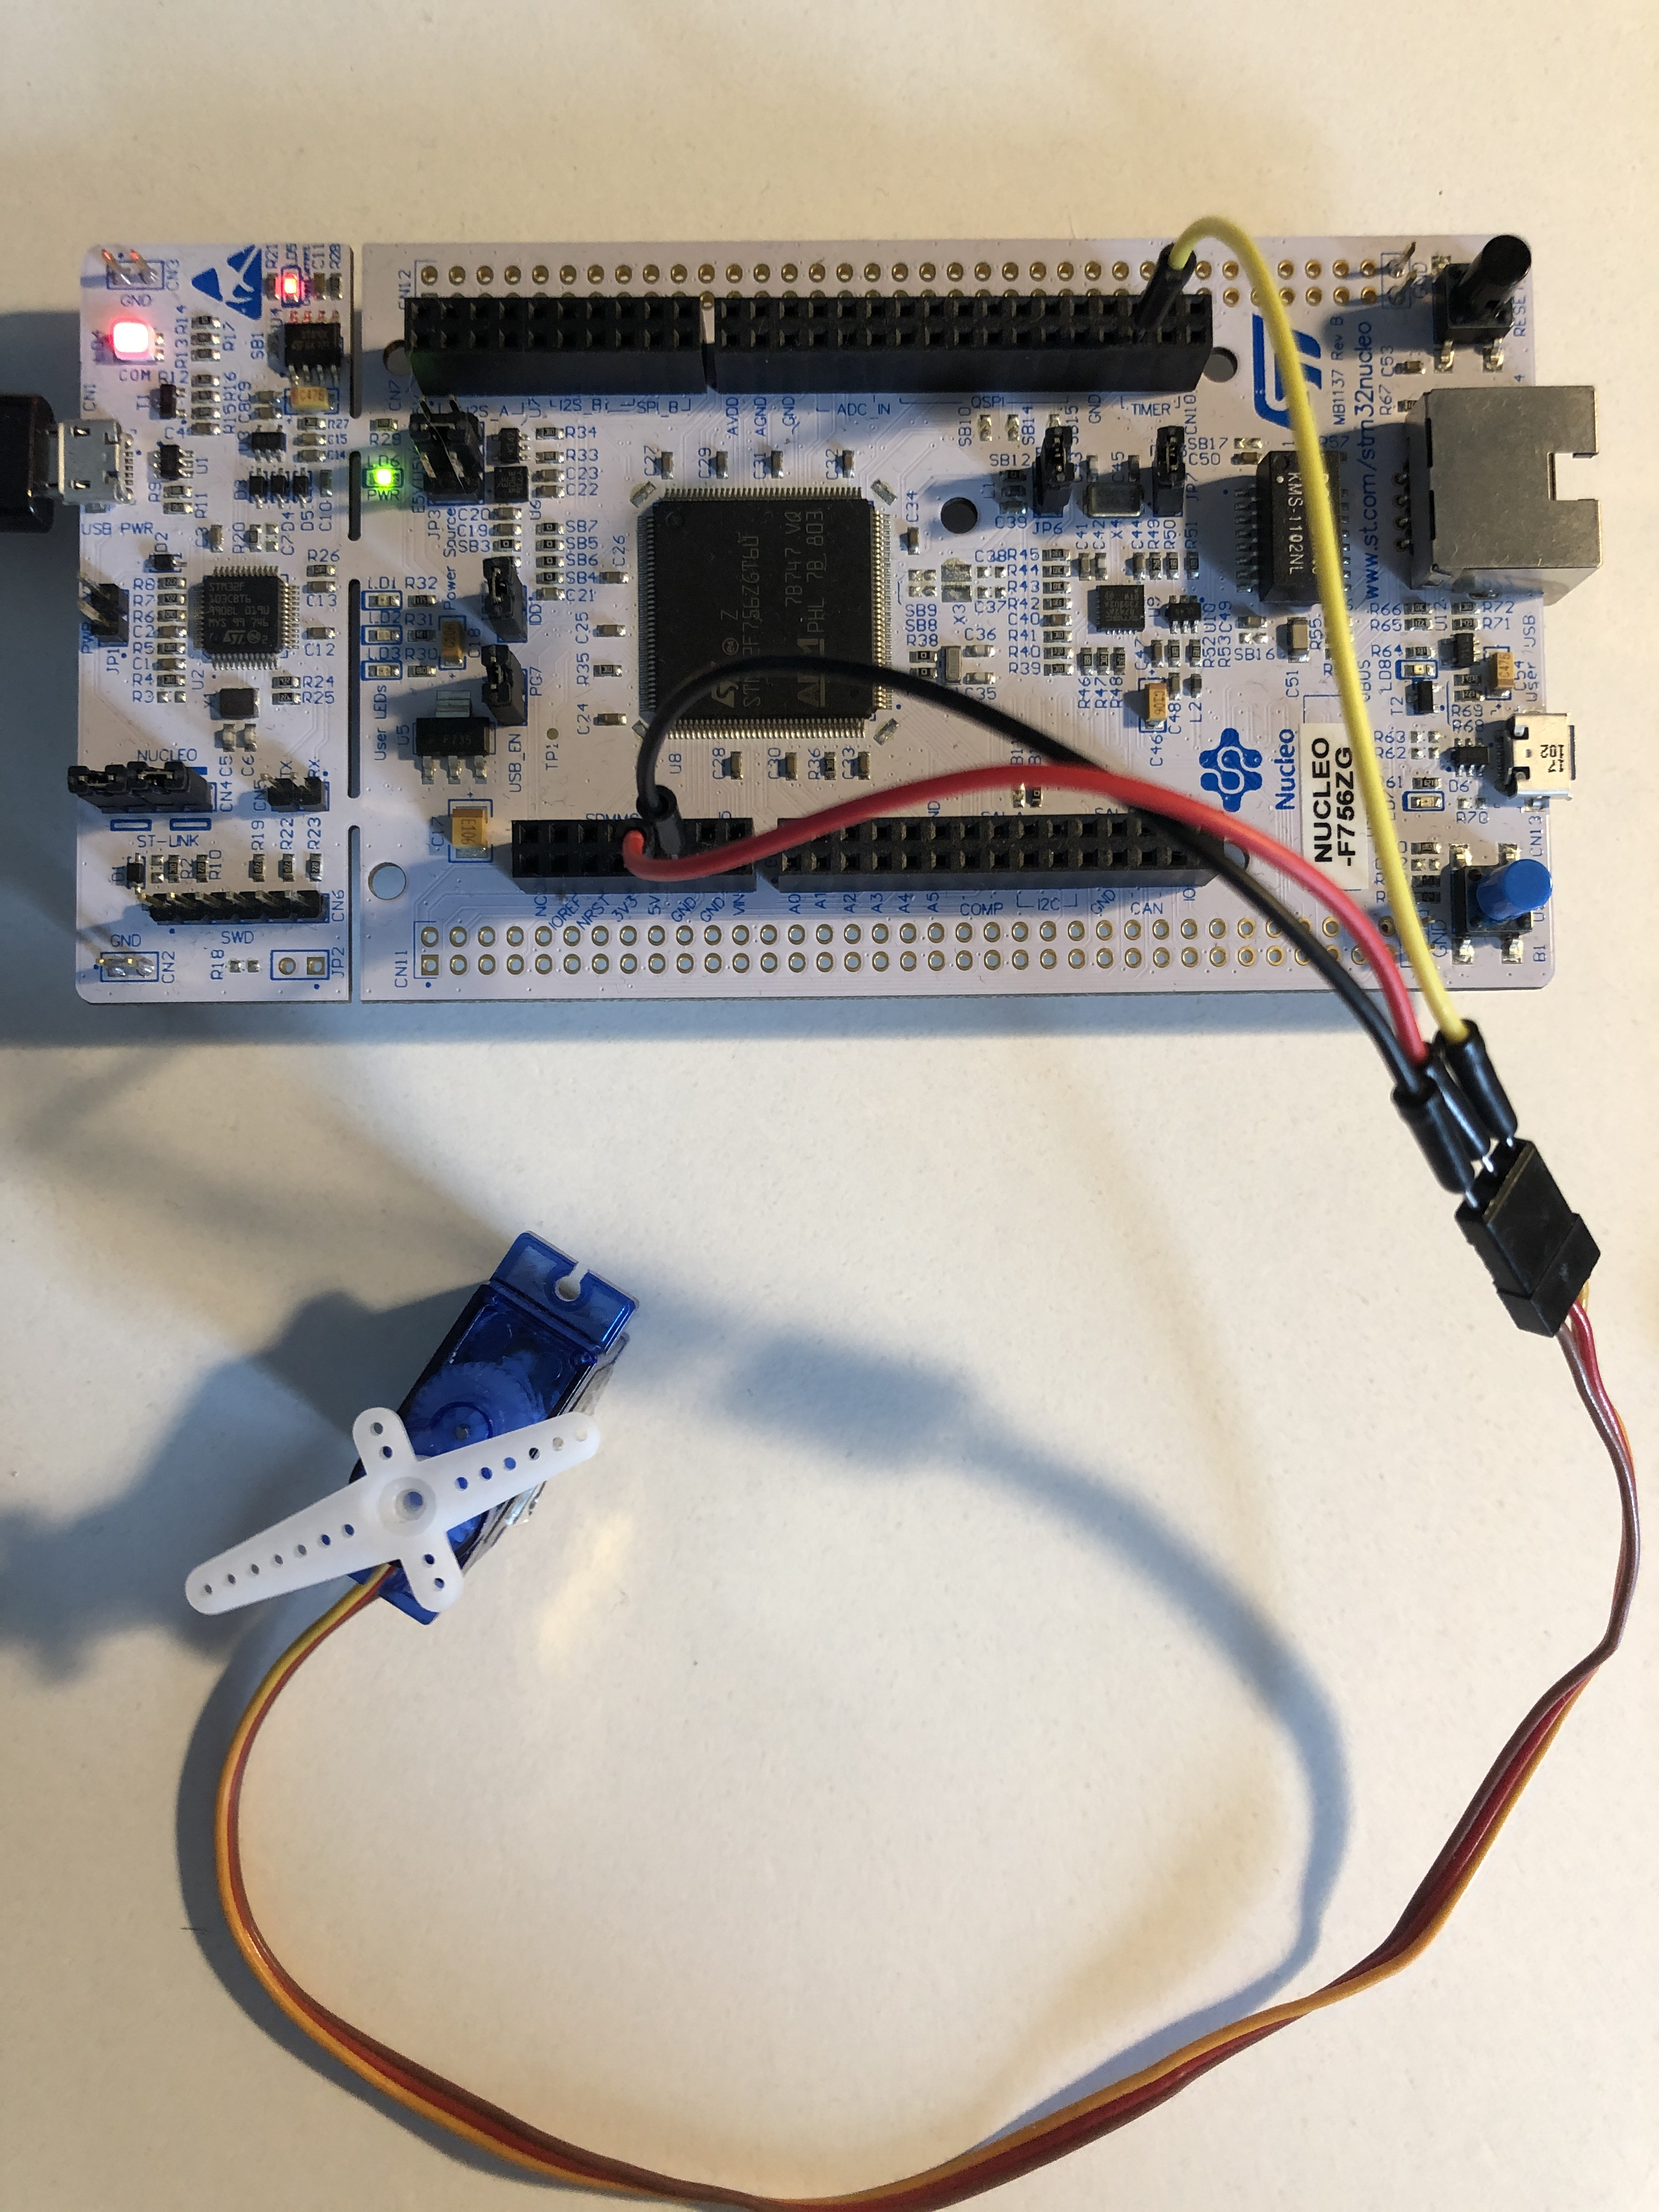
\includegraphics[width=0.45\textwidth,angle=90,origin=c]{fig/Serwo/polaczenie_modulu/podlaczenie.jpg}
    \caption{Działanie fotorezystora przy dużym natężeniu światła}
    \label{fig:my_label}
\end{figure}

Po zaprogramowaniu mikrokontrolera w środowisku CubeIDE możliwe jest dowolne zadawanie pozycji serwomechanizmu za pomocą wypełnienia PWM; przedstawione na zdjęciach zostały dwie skrajne pozycje - 0$^{\circ}$ oraz 180$^{\circ}$.

\begin{figure}[h!]
\centering
\begin{subfigure}{.5\textwidth}
  \centering
  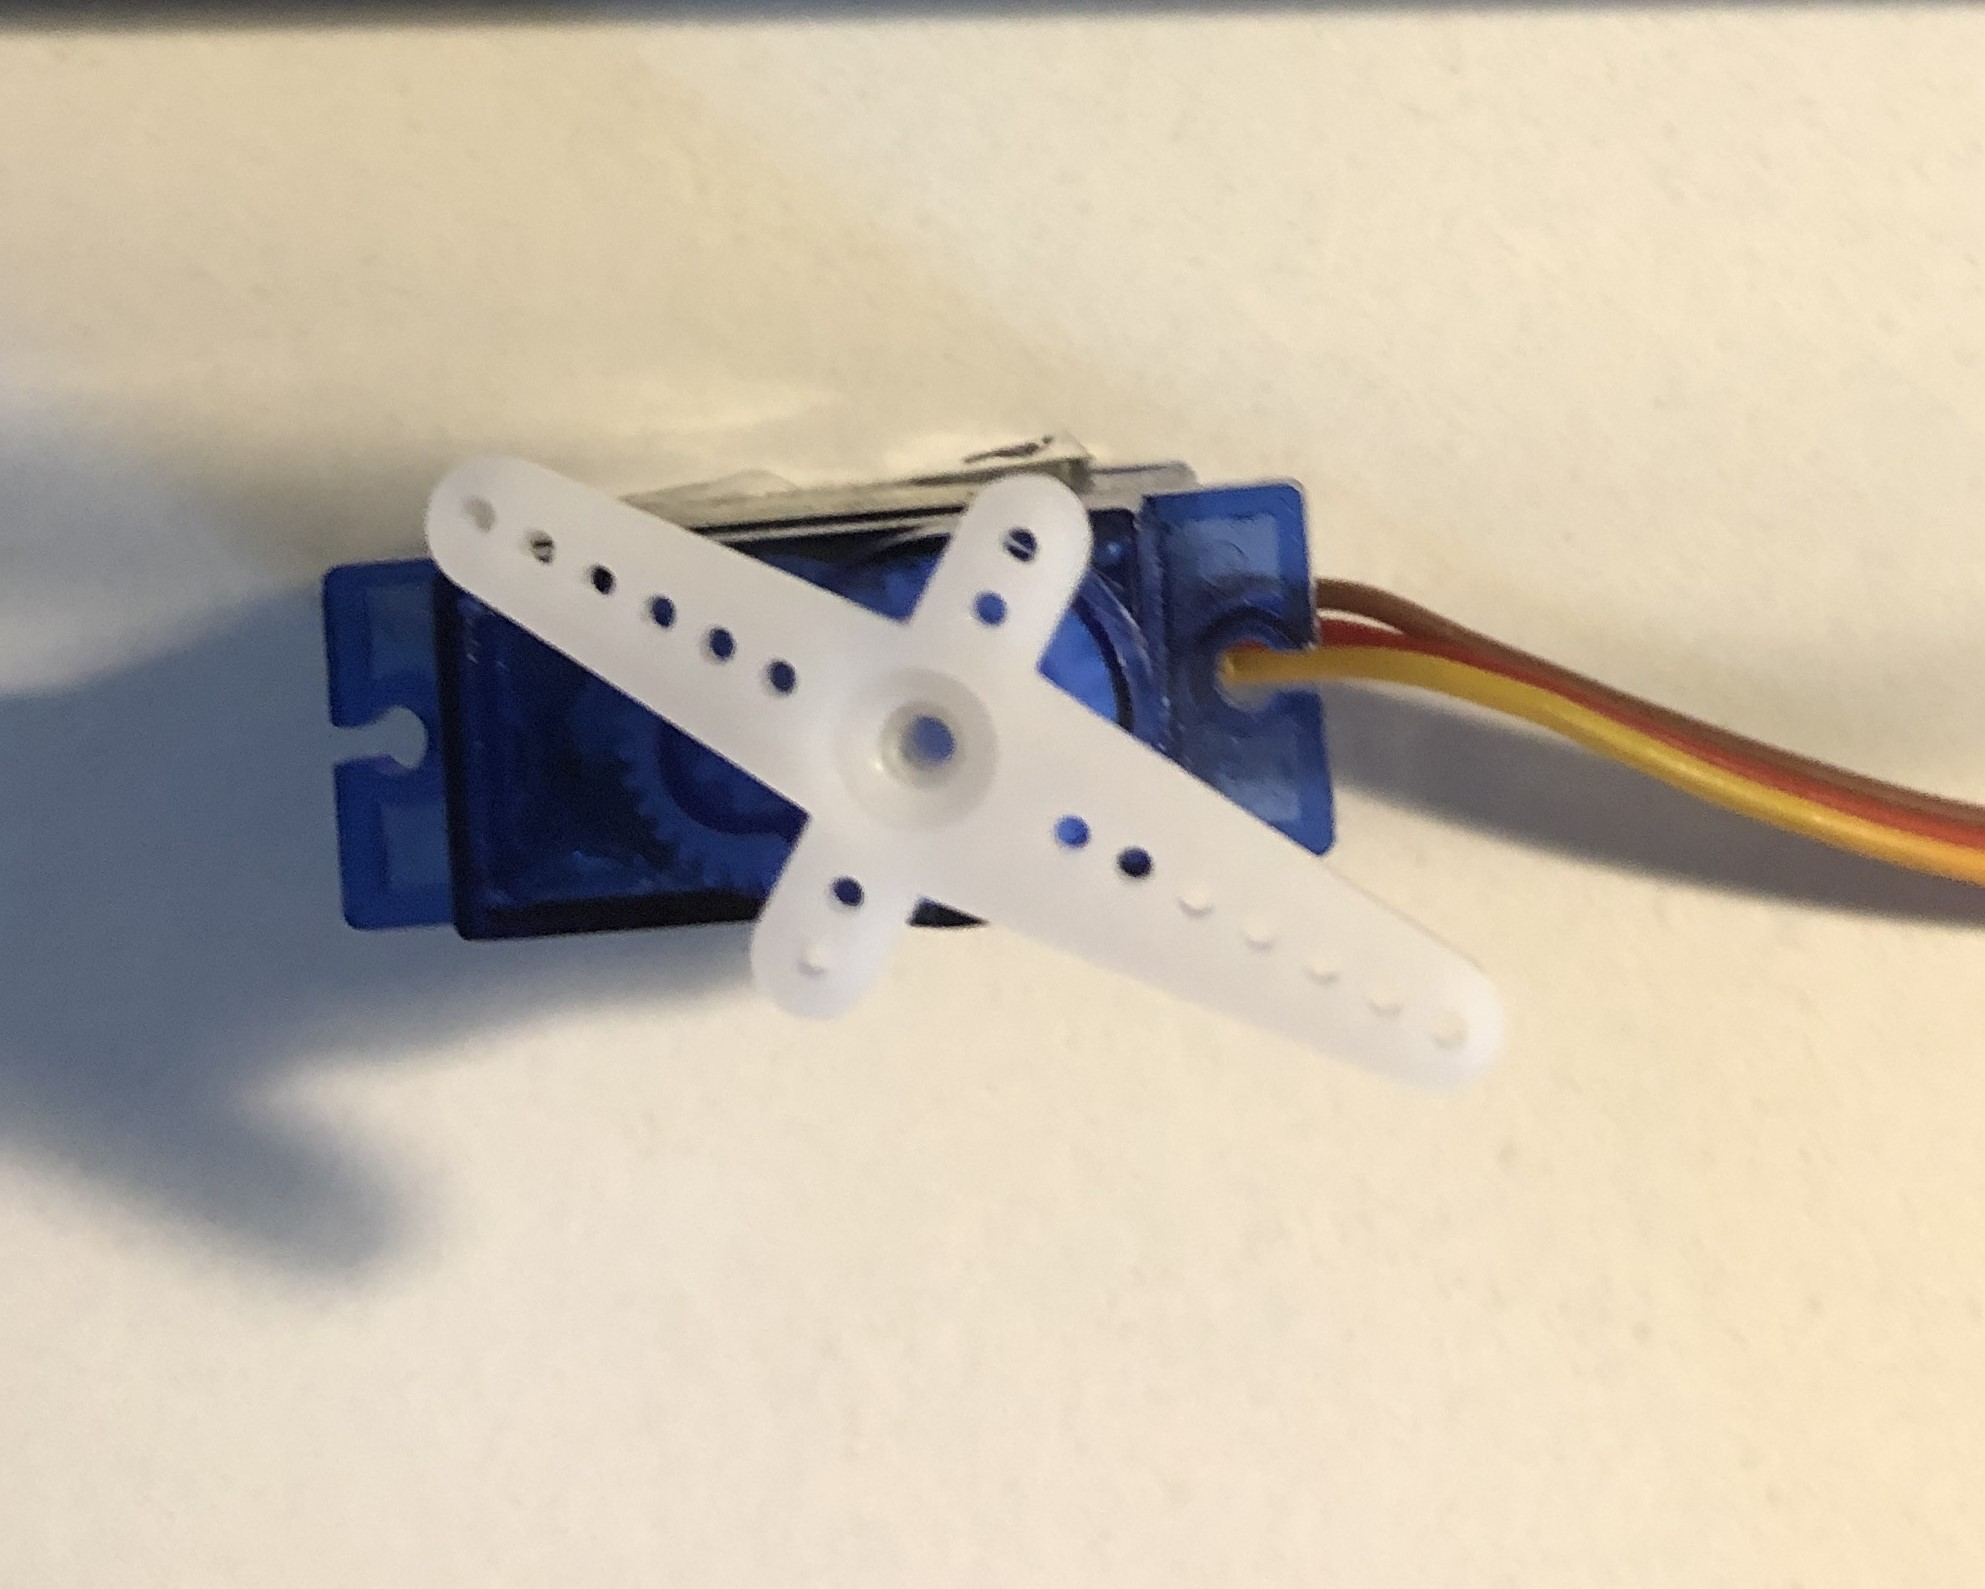
\includegraphics[width=0.9\linewidth]{fig/Serwo/zasada_dzialania/0.jpg}
  \caption{Wychylenie 0 stopni}
  \label{fig:sub1}
\end{subfigure}%
\begin{subfigure}{.5\textwidth}
  \centering
  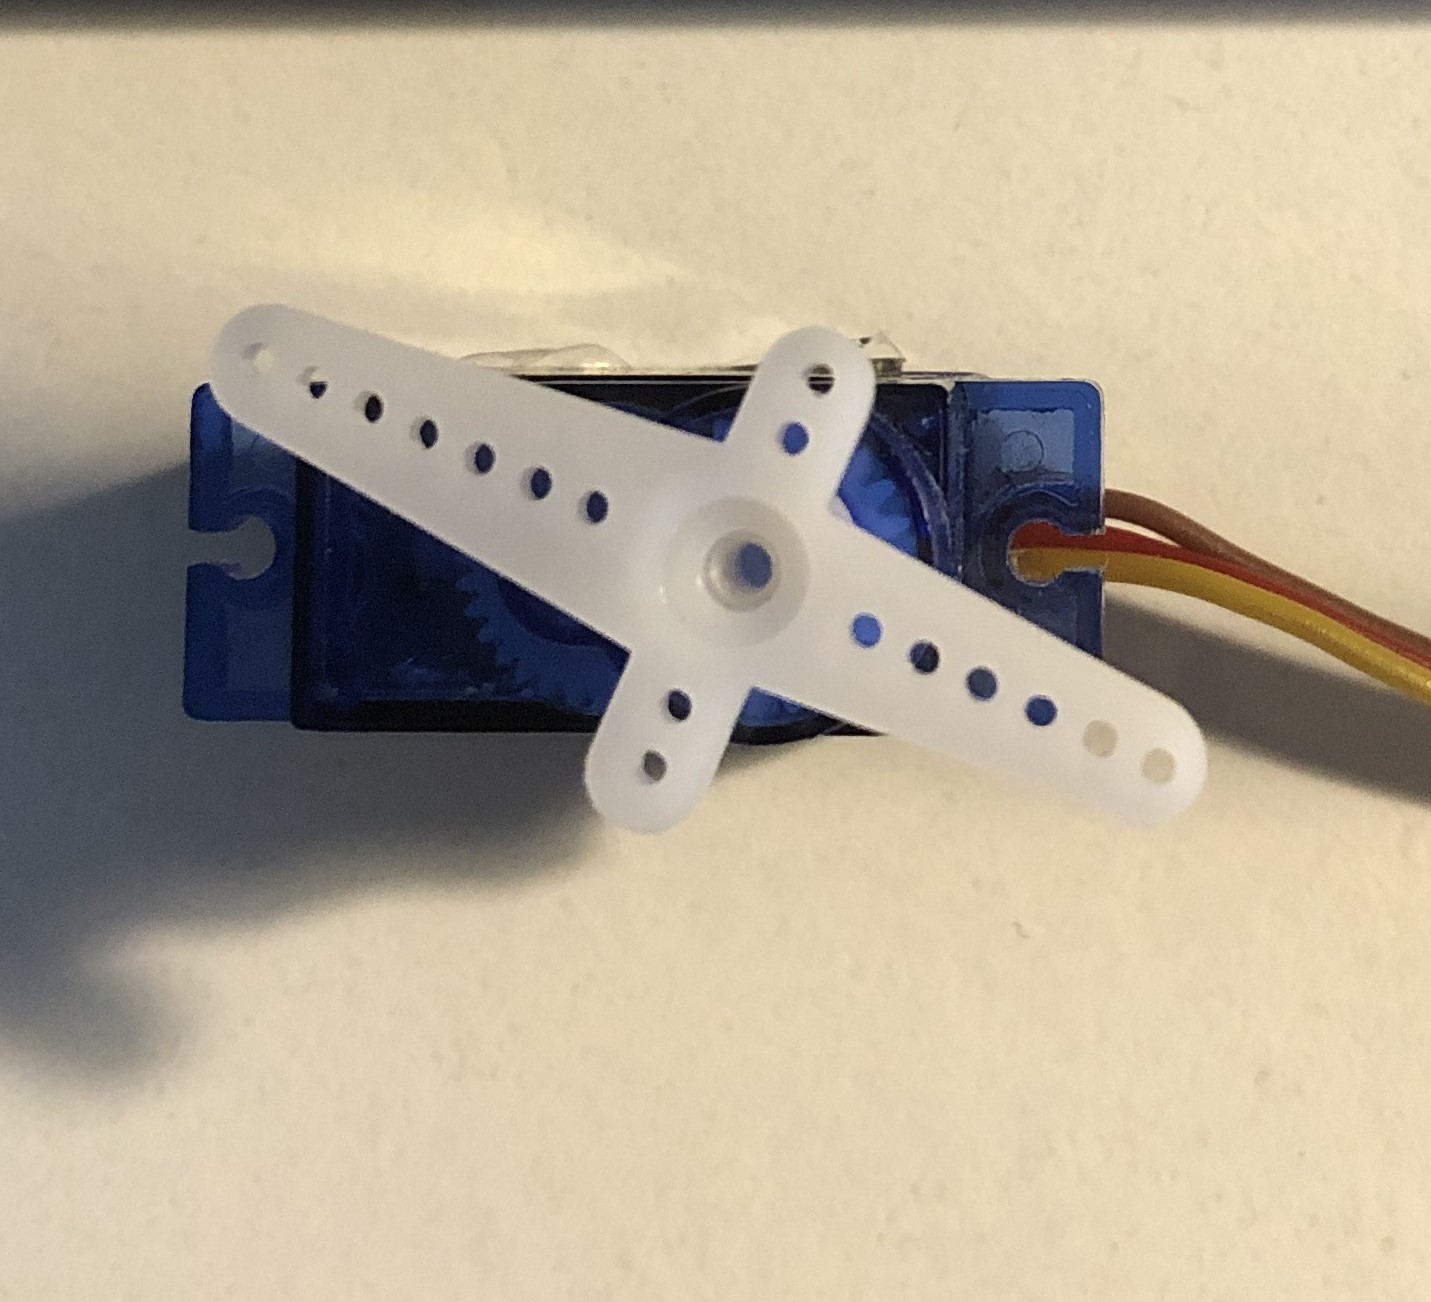
\includegraphics[width=0.78\linewidth]{fig/Serwo/zasada_dzialania/180.jpg}
  \caption{Wychylenie 180 stopni}
  \label{fig:sub2}
\end{subfigure}
\caption{Skrajne wartości obrotu}
\label{fig:test}
\end{figure}
\newpage


Kod programujący czujnik, wykorzystany do opracowania instrukcji, znajduje się w materiałach dodatkowych zawartych pod koniec rozdziału.
\newline
Film prezentujący działanie układu znajduje się w suplemencie wideo.
\printbibliography[heading=bibintoc]

\end{document}